\documentclass{beamer}

\mode<presentation> {
\usetheme{Madrid}
}

\usepackage{graphicx} % Allows including images
\usepackage{booktabs} % Allows the use of \toprule, \midrule and \bottomrule in tables
\usepackage{hyperref}
\usepackage{color}

\newcommand{\ut}[1]{\ensuremath{\tilde{#1}}}

%----------------------------------------------------------------------------------------
%	TITLE PAGE
%----------------------------------------------------------------------------------------

\title[Recycle Robot]{Motion Planning for Recycling Robotics: Progress Report} % The short title appears at the bottom of every slide, the full title is only on the title page

\author[Link, Tormey, LeVan]{Nicholas Link, Samuel Tormey, Ricky LeVan} % Your name

\date{\today} % Date, can be changed to a custom date

\begin{document}

\begin{frame}
\titlepage % Print the title page as the first slide

\end{frame}

\begin{frame}
\frametitle{Intro}
\begin{itemize}
\item We are building a simulated robot to manipulate objects on a conveyor belt
\item We were motivated by the desire to improve recycling efficiency
\end{itemize}
\begin{centering}
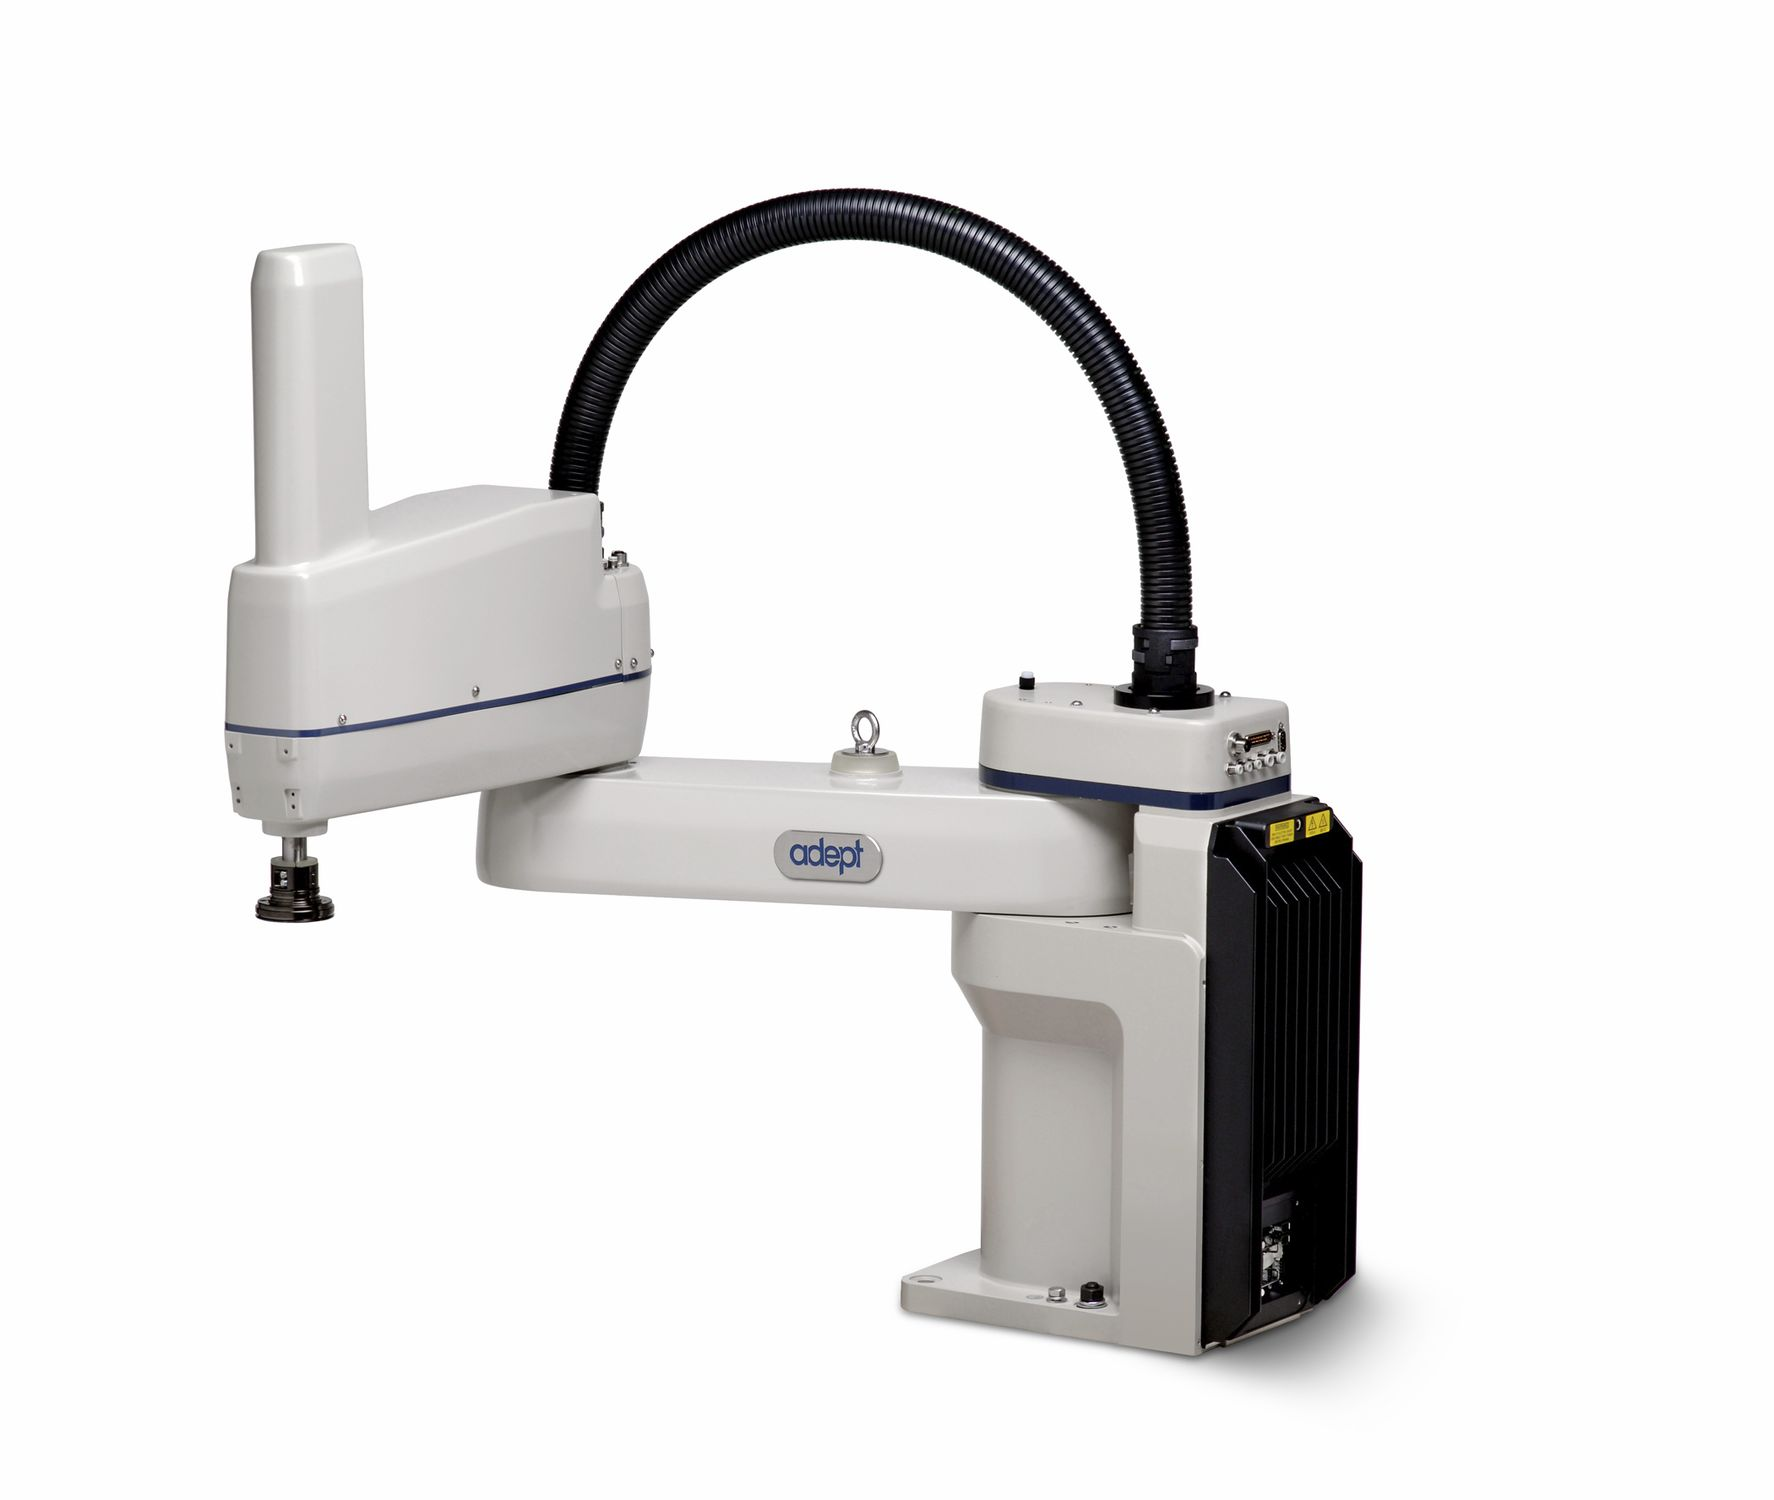
\includegraphics[width=0.55\linewidth,height=0.55\textheight,keepaspectratio]{scara.jpg}

\end{centering}

\end{frame}


\begin{frame}
\frametitle{Review: Last Semester's Work}
\begin{itemize}
\item First we researched the robot dynamics for a SCARA arm.

\item Next we formulated our optimization problem:
\begin{align*}
\min  & \: \:T \\
\mbox{s.t. } & \frac{d\ut{x}(\tau)}{d\tau} = Tf(\ut{x}(\tau),\ut{u}(\tau))  &\tau \in [0,1] \\
& -M \leq \ut{u}_j(\tau) \leq M  & 1 \leq j \leq 3 \\
& \ut{x}(0) = x_0 \\
& \ut{x}(1) = x_{\scriptsize\mbox{T}} 
\end{align*}

\end{itemize}

\end{frame}


\begin{frame}
\frametitle{Outline of current and future work}
Current work:
\begin{itemize}
\item Custom Jacobian
\item 3D robot animation
\end{itemize}
Future work:
\begin{itemize}
\item Online optimal path finding
\item Temporal goal planning
\end{itemize}

\end{frame}

\begin{frame}
\frametitle{Custom Jacobian}
Reminder: Our dynamics can be written in the following form:
$$b = \frac{x_{i+1} - x_i}{d\tau} - Tf(x_i,u_i) = 0$$
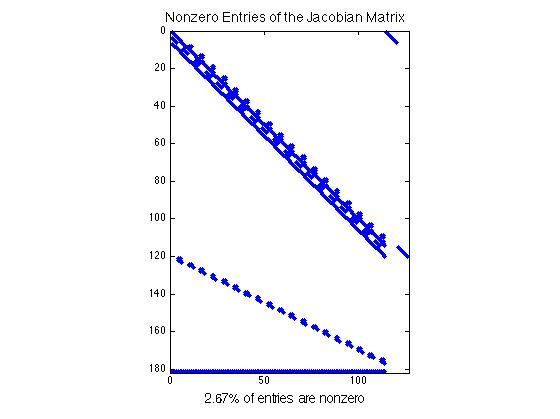
\includegraphics[width=0.75\linewidth,height=0.55\textheight]{Spy_Jacobian.jpg}

\end{frame}


\begin{frame}
\frametitle{3-D Robot Animation}
Here is a video of our current simulation

\end{frame}

\begin{frame}
\frametitle{Online performance}
\begin{itemize}
\item A key component is efficiently generating an initial guess
\item We may consider pre-computing optimal paths
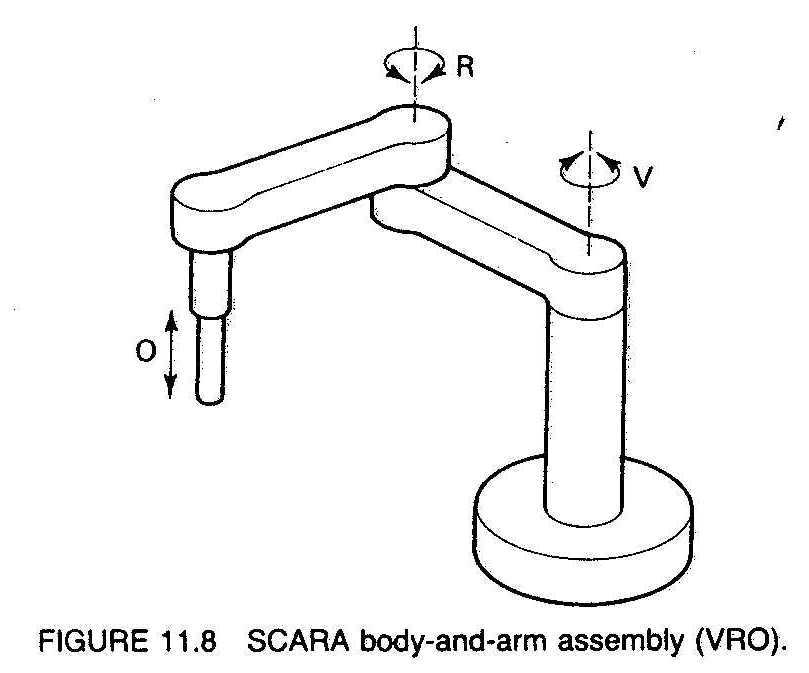
\includegraphics[width=0.55\linewidth,height=0.55\textheight,keepaspectratio]{scara2.jpg}


\end{itemize}

\end{frame}

\begin{frame}
\frametitle{Temporal Goal Planning}
\begin{itemize}
\item Currently, our system finds an optimal path, grabs and moves an object, then repeats.
\item With temporal goal planning, we can search several steps in advance for a more 
globally optimal solution
\end{itemize}

\end{frame}



\end{document}

